\documentclass[12pt, twoside]{article}
\usepackage[text={16cm,23cm},centering]{geometry}
\usepackage{booktabs}
\usepackage[table,xcdraw]{xcolor}
\usepackage{graphicx}
\usepackage{listings}
\usepackage{xcolor}
\lstset{basicstyle=\ttfamily,language=c,keywordstyle=\color{blue}}
\usepackage{amsmath}
\usepackage{hyperref}
\usepackage{svg}
\usepackage{subcaption}

\setlength{\parskip}{1.2ex}
\setlength{\parindent}{0em}
\clubpenalty = 100
\widowpenalty = 100

\begin{document}

\title{Raytracer accelerato via CUDA}

\author{Marco Cutecchia, 983828}

\date{}

\maketitle

\section{Introduzione}
Il raytracing è una tecnica utilizzata in computer grafica per il rendering
di immagini realistiche che consiste nel simulare il modo in cui la luce
interagisce nel mondo.
L'ispirazione principale viene dalle fotocamera \textit{pinhole}:
in questo modello i raggi di luce entrano in una \textit{camera oscura}
tramite un piccolo buco in uno dei lati della camera.
Il risultato è che l'immagine puntata viene proiettata ribaltata sul
lato opposto al buco.

In una fotocamera reale avremmo bisogno di sensori per catturare la luce che
arriva nel piano, in un raytracer mapperemo questo piano all'immagine finale,
assegnando ad ogni pixel il colore dei raggi che colpiscono la sua area nel
piano.
Essendo il piano virtuale all'interno di un raytracer, possiamo anche spostarlo
per essere davanti al pinhole, dove l'immagine non è più ribaltata

\begin{figure}[h]
  \centering
  \begin{subfigure}{.4\textwidth}
    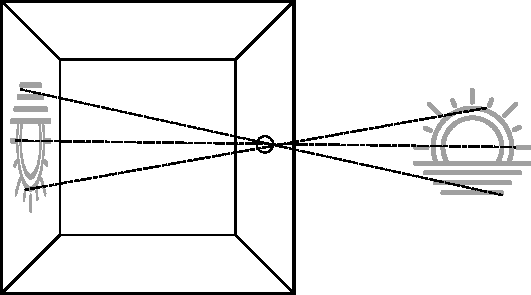
\includegraphics[width=\linewidth]{images/PinholeCamera.pdf}
  \end{subfigure}
  \hspace{0.1\textwidth}
  \begin{subfigure}{.4\textwidth}
    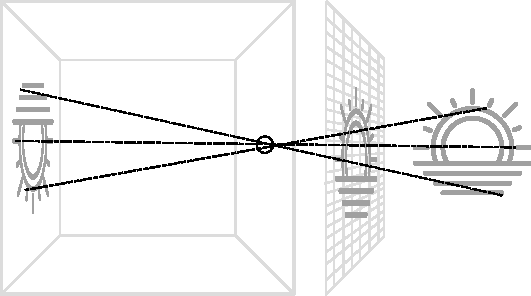
\includegraphics[width=\linewidth]{images/PinholeFocalPlane.pdf}
  \end{subfigure}
\end{figure}

Simulare il comportamento di tutti i raggi in una scena è estremamente
difficile e neanche utile visto che ci interessano solamente i raggi di luce
che riescono ad entrare nella nostra camera oscura.
Una tecnica molto comune nel mondo del raytracing consiste dunque nel simulare
il percorso di questi raggi al contrario, questo ci permette dunque di
considerare solamente i raggi che sappiamo essere passati per il buco della
nostra fotocamera (e dunque utili ai fini del generare l'immagine). 

Nonostante questa ottimizzazione il raytracing rimane comunque difficile da
implementare in contesti di grafica real-time a causa del grande numero di
raggi da simulare, è però molto popolare nel rendering offline; inoltre è un
problema che si presta molto bene alla parallelizzazione dato che il calcolo
per ognuno dei raggi da simulare è completamente indipendente dagli altri.

Il raytracer implementato in questo report è in parte basato su quello
descritto nel libro \textit{Raytracing in One Weekend}\cite{raytracingin1weekend}, dove
viene implementata una versione single-thread su CPU.
Più nel dettaglio è un \textit{path-tracer}, cioè per ogni pixel proietta più
raggi facendone la media del colore, applicando un leggerissimo shift
randomizzato sull'origine dei raggi.
Il raytracer permette di renderizzare scene composte da sfere di materiale
opaco (con texture o senza), metallo o dielettrico.
Per la conversione da array di pixel \texttt{ARGB} a immagine \texttt{png}
è stata utilizzata la libreria \texttt{stb\_image\_write}\cite{stb}. 

L'immagine qui di seguito è stata prodotta dal mio raytracer:

\begin{figure}[h]
  \centering
  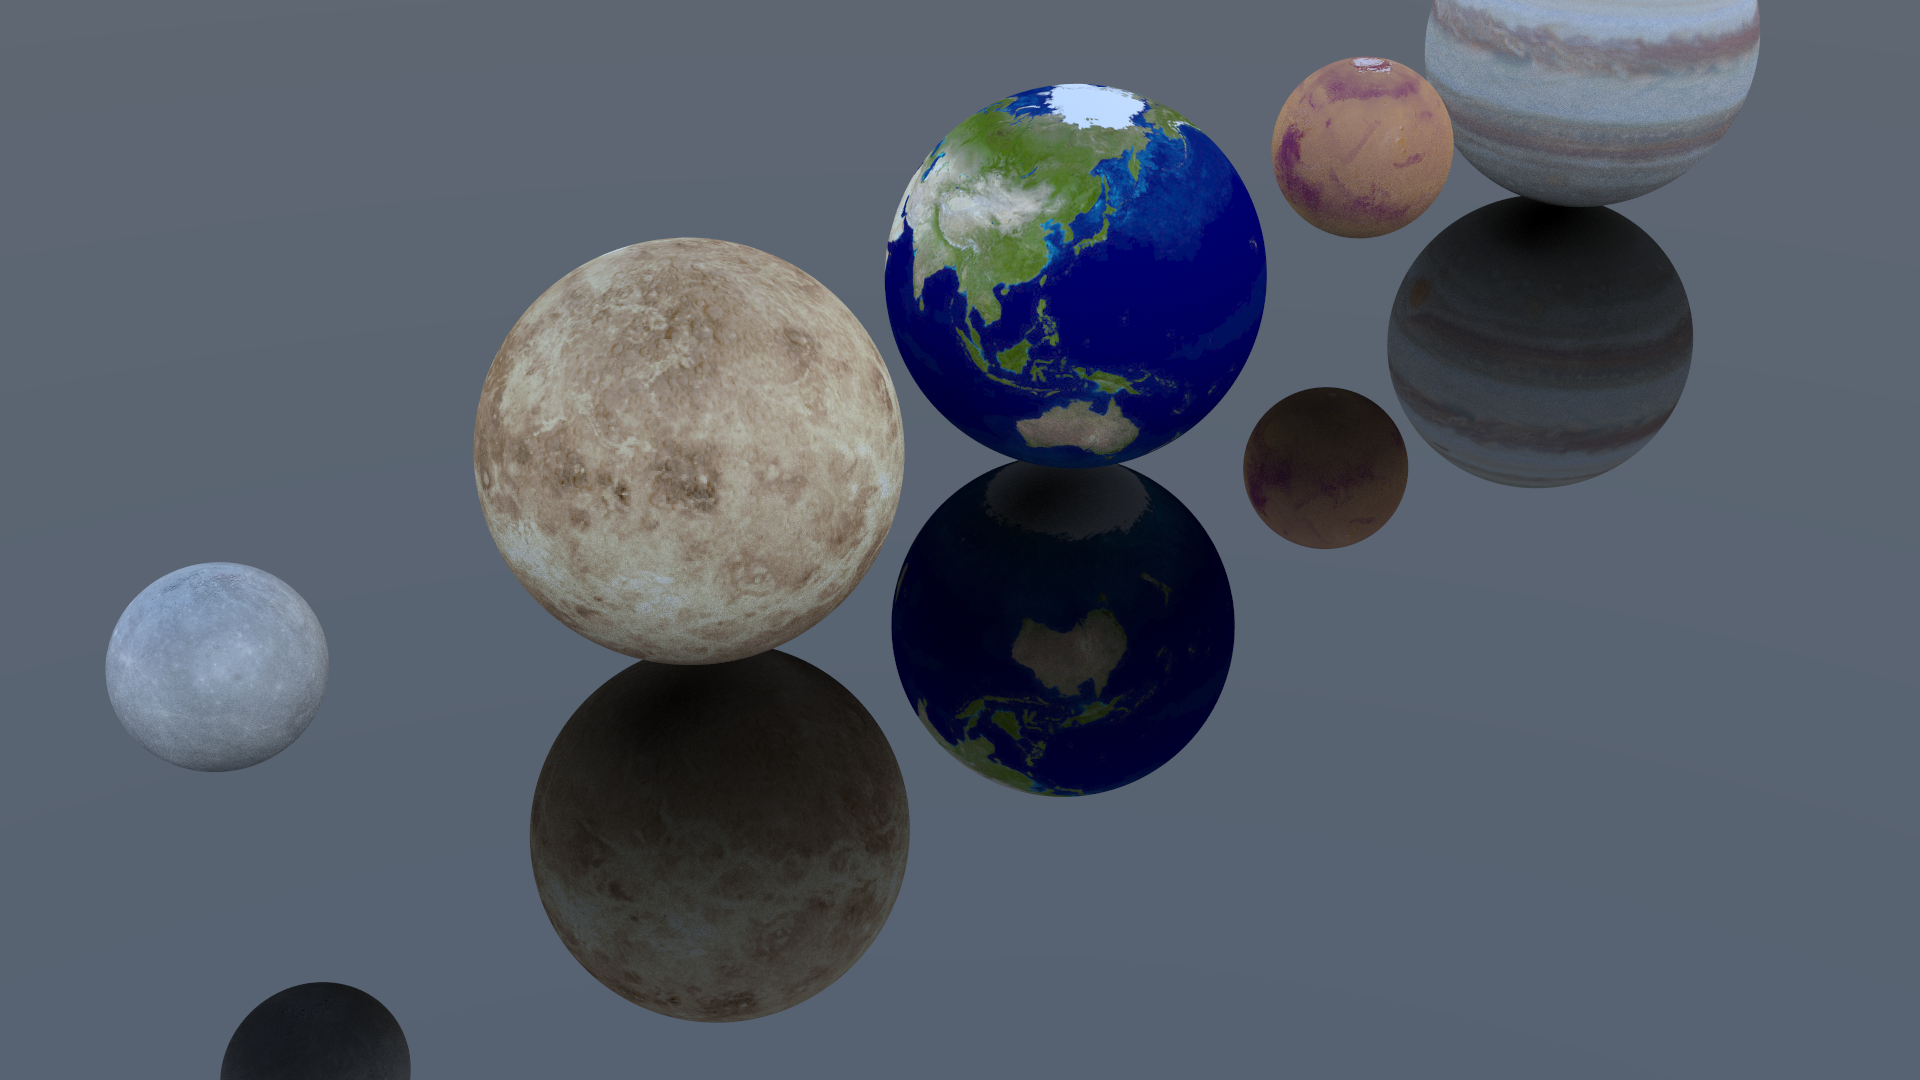
\includegraphics[width=\linewidth,keepaspectratio]{images/renders/planets.png}
\end{figure}

\section{Algoritmo del raytracing}
Alla base del raytracing sta il concetto di \textit{raggio}; un raggio è
semplicemente una retta in uno spazio tridimensionale, dunque possiamo
esprimere i punti su di essa con la semplice formula $P(t) = A + B \cdot t$.

Possiamo definire questi raggi anche tramite due punti per cui passano: il
primo punto è il buco della nostra fotocamera, una costante che chiameremo
$CameraPos$ nelle formule in avanti, l'altro è un punto sul
\textit{piano focale} o \textit{vista}.
Questa vista è il muro sulla quale viene proiettata l'immagine all'interno
della nostra fotocamera, spostato però davanti al buco.
Dato un punto di coordinate $(x, y)$ nell'immagine finale allora il suo
corrispondente nello spazio 3D sul piano sarà dato da:

$$
  \frac{x}{ImageWidth} \cdot ViewWidth \cdot H + \frac{y}{ImageHeight} \cdot ViewHeight \cdot V + LowerLeftCorner
$$

In questa formula $H$ e $V$ sono due vettori unitari che puntano nelle
direzioni per muoversi orizzontalmente e verticalmente sul piano
(per esempio $H=(1, 0, 0)$ e $V=(0, 1, 0)$) mentre il resto delle variabili,
eccetto $x$ e $y$, sono parametri di configurazione per variare l'aspetto
dell'immagine finale.
Idealmente il rapporto $\frac{ViewWidth}{ViewHeight}$ è uguale a quello di
$\frac{ImageWidth}{ImageHeight}$, altrimenti l'immagine finale verrà
schiacciata o allungata.

\bigbreak

La dimensione e posizione del piano rispetto alla telecamera influenzano
quanti raggi catturati dal pinhole finiranno poi nella immagine finale.
Il piano focale può essere descritto tramite due variabili: la
\textit{lunghezza focale}(o \textit{focal length}) e
l'\textit{angolo di visione}(o \textit{field of view}, \textit{FoV}).
La lunghezza focale è la distanza tra telecamera e piano
mentre l'angolo di visione, che può essere orizzontale o verticale (è una
preferenza), implica quanta luce entra nel pinhole.
Un piano molto grande e vicino al pinhole implica che molti più raggi finiscono
per intersecare il piano e dunque una porzione di scena maggiore è visibile,
al contrario un piano molto piccolo alla stessa distanza catturerà raggi in
una area molto più piccola, il risultato è un effetto zoom.

Il variare della lunghezza focale può avere anche degli effetti sulla messa
a fuoco dell'immagine quando si ha una lente curva in una fotocamera, in questo
raytracer però non simuliamo una lente dunque non ci interessa.

\begin{figure}[h]
  \centering
  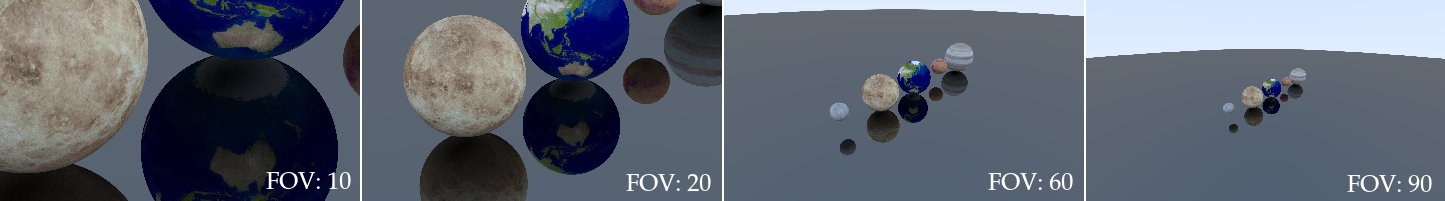
\includegraphics[width=\linewidth,keepaspectratio]{images/fov_changes.png}
\end{figure}

Questi due parametri descrivono il piano sulla quale viene proiettata
l'immagine:
assumendo un $FoV$ verticale ed una distanza focale di $1$ allora l'altezza
del piano sarà data da $ViewHeight = tan(\frac{Fov}{2})$ mentre la larghezza
sarà $ViewWidth = ViewHeight \cdot AspectRatio$ dove
$AspectRatio = \frac{ImageWidth}{ImageHeight}$.
Il centro del piano si troverà dunque alle coordinate
$(0, 0, 1)$ e l'angolo in basso a sinistra sarà:

$$
  LowerLeftCorner = (0, 0, 1) - \frac{ViewWidth}{2} - \frac{ViewHeight}{2}
$$

Un raytracer, per ogni pixel dell'immagine, proietta uno o più raggi, con
associato un colore iniziale per ciascuno ed osserva il colore finale di
ogni raggio dopo che questi vanno a collidere con eventuali oggetti nella
loro traiettoria dalla telecamera al piano.
Il materiale di cui sono fatti gli oggetti con cui un raggio va a collidere
determina il modo in cui il colore del raggio viene modificato: per esempio un
materiale opaco assorbe una parte di luminosità del raggio.

Il seguente pseudocodice mostra il "cuore" di un raytracer, seppur nasconda
alcuni aspetti importanti come un modo per trovare l'intersezione tra raggio
e oggetti e la \textit{funzione di trasporto del colore} dei materiali: il
motivo è semplicemente che questi aspetti dipendono dalla scena che vogliamo
renderizzare.

\newpage

\begin{lstlisting}[mathescape=true]
    for (int x = 0; x < ImageWidth; x++) {
      for (int y = 0; y < ImageHeight; y++) {
        Sia $\textbf{p}$ il punto sul piano corrispondente al
          pixel (x, y)
        Sia $\textbf{r}$ una retta che passa per i punti
          $\textbf{CameraPosition}$ e $\textbf{p}$
        Sia $\textbf{o}$ il primo oggetto che interseca la retta $\textbf{r}$
          partendo da $\textbf{CameraPosition}$ in avanti

        if (la retta $\textbf{r}$ non interseca oggetti) then {
          Il pixel (x, y) ha colore dello sfondo
        } else {
          Sia $\textbf{m}$ il materiale di cui è composto $\textbf{o}$
          Sia $\textbf{c}$ il colore ottenuto applicando la funzione
            di dispersione di colore del materiale $\textbf{m}$ al
            colore dello sfondo
          
          Il pixel (x, y) ha colore $\textbf{c}$
        }
      }
    }
\end{lstlisting}

\subsection{Calcolo dell'intersezione tra un raggio ed una sfera}
Per trovare se la retta $r$ interseca con qualche oggetto una possibile
soluzione è quella di iterare su tutti gli oggetti della scena e, utilizzando
qualche formula geometrica, calcolare il punto di intersezione tra l'oggetto
e la retta (se esiste).
L'oggetto con il punto di intersezione con distanza minore dalla telecamera è
quello il cui materiale deve essere usato per determinare il colore del raggio.

Per esempio se volessimo calcolare l'intersezione tra una retta ed una sfera
di raggio $r$ centrata in $C$ potremmo osservare che i punti su una sfera sono
descritti dall'equazione:

$$
    (x - C_x)^2 + (y - C_y)^2 + (z - C_z)^2 = r^2
$$

Che possiamo scrivere anche in questo modo:

$$
    r^2 = (P - C) \cdot (P - C)
$$

I punti del nostro raggio sono descritti dalla funzione $P(t)=A + t \cdot b$,
vogliamo dunque trovare se esistono dei punti su $P(t)$ che soddisfano anche
l'equazione.
Sostituiamo dunque a $P$ l'equazione della nostra retta e, dopo un po' di
semplificazioni matematiche, otteniamo una equazione di secondo grado:

$$
  (A + t \cdot B - C) \cdot (A + t \cdot B - C) = r^2
$$
$$
  t \cdot 2b^2 + t \cdot 2b (A-C) + (A-C) \cdot (A-C) - r^2 = 0
$$

In questa equazione l'incognita $t$ sono i punti di intersezione, è possibile
risolverla con la classica formula $\frac{-b +- \sqrt{b^2 - 4ac}}{2a}$.
In base al numero di soluzioni trovate possiamo capire se il raggio non
interseca la sfera (zero soluzioni trovate, discriminante negativo), se la
retta passa tangente per un solo punto (una sola soluzione, discriminante
uguale a zero) oppure se la retta attraversa la sfera e dunque ci sono due
punti di intersezione; in quest'ultimo caso sceglieremo la soluzione con
distanza minore dalla telecamera.

\begin{figure}[h]
  \centering
  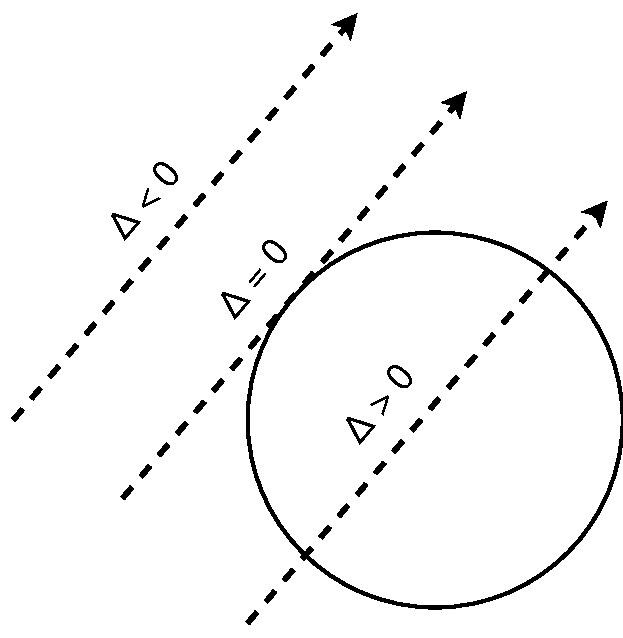
\includegraphics[width=0.3\linewidth,keepaspectratio]{images/SphereRayIntersection.pdf}
\end{figure}

\subsection{Calcolo della funzione di trasporto del colore di un materiale opaco}

Calcolare accuratamente la funzione di trasporto del colore può essere spesso
molto difficile, questo perchè potrebbe dipendere da talmente tanti altri
elementi al punto da dover simulare l'intero universo.
Per questo motivo nella realtà quello che facciamo è utilizzare un modello
molto più semplice che però da risultati visivi simili.
Il modello che andiamo a descrivere è un approssimazione molto grossolana del
modello delle superfici \textit{Lambertiane}, un tipo di materiale che riflette
luce in modo uguale su tutta la sua superficie.

In questo modello un materiale opaco prende il suo colore mischiando il suo
colore innato (detto \textit{albedo}) a quello ottenuto dai materiali riflessi
su di esso.
Dato un raggio che interseca questo materiale il suo colore è dato dall'albedo
del materiale (rappresentato come un vettore a 3 dimensioni di valori
$RBG$ tra $[0, 1]$) moltiplicato componente per componente con il colore di un
raggio riflesso.
Questo raggio riflesso è descritto da due punti: il punto di intersezione del
raggio precedente e il vettore normale della superficie.

\begin{figure}[h]
  \centering
  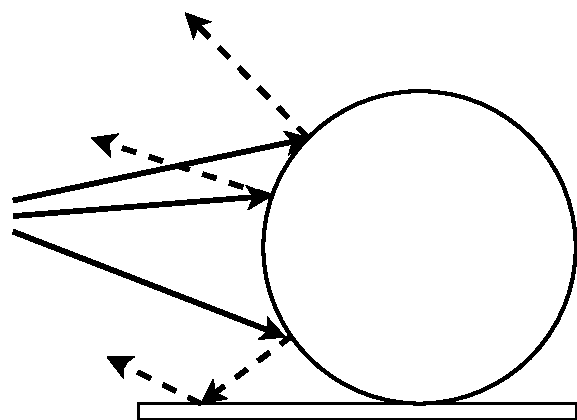
\includegraphics[width=0.3\linewidth,keepaspectratio]{images/LambertianRayReflection.pdf}
\end{figure}

Per esempio, se determiniamo che il nostro raggio colpisce una sfera nella
posizione $P$ e l'albedo del materiale è rosso $(0.7, 0, 0)$, allora per
calcolare il colore del raggio dovremo prima determinare ricorsivamente il
colore di un raggio che parte da $P$ ed ha come direzione il vettore normale
alla curva e poi moltiplicare questo colore per l'albedo del materiale,
in questo caso $(0.7, 0, 0)$.

Per determinare il vettore normale alla superficie di una sfera basta
sottrarre al punto $P$ il punto origine della sfera e normalizzare il
vettore. 
Nota che questo metodo per calcolare la normale restituisce sempre un
vettore che punta "al di fuori" della sfera, dunque non sarebbe corretto
se volessimo simulare di essere noi spettatori dentro una sfera di questo
materiale.

\section{Accelerazione via GPU}
Per accelerare via CUDA questo processo l'immagine finale è stata divisa in
blocchi rettangolari $8 x 4$, ogni thread si occupa di un singolo pixel
dell'immagine finale e proietta un raggio associato a quel pixel.
La scelta di queste dimensioni è data dal voler ottenere una dimensione dei
blocchi multipla di $32$ per utilizzare al massimo ogni warp e da test
empirici, dove queste dimensioni hanno permesso di avere le performance
migliori.

Prima di iniziare il rendering vengono caricate in \textit{constant memory}
diversi oggetti che vengono utilizzati da tutti i thread.
Esempi di questi dati sono i parametri della camera e gli elementi della
scena, che includono gli oggetti e i loro materiali associati.

Il raytracer implementato fa parte della categoria dei \textit{path tracer},
cioè per ogni pixel vengono proiettati più raggi e viene fatta la media dei
colori ottenuti.
Ad ogni raggio viene applicato uno leggero shift randomizzato alla direzione,
questo permette di ottenere delle ombre più "leggere".
Il numero di raggi proiettato per ogni pixel è un parametro configurabile,
detto \textit{samples per pixels}; di solito oltre i $100$ raggi per pixel
l'effetto diventa meno evidente.

Il calcolo di questi raggi può essere svolto in modo parallelo, per fare
questo l'immagine è divisa in una grid a 3 dimensioni, dove la $z$ indica
l'indice del raggio calcolato per un singolo pixel.
Tutti i thread, dopo aver determinato il colore del proprio raggio, effettuano
una somma vettoriale del proprio colore con tutti gli altri thread per quel
pixel sopra il framebuffer.
Questa somma è fatta in modo atomico con la funzione \texttt{atomicAdd}.

I thread scrivono il colore calcolato del raggio che hanno proiettato su un
framebuffer allocato in device memory; questo è un framebuffer contenente i
valori RGB espressi come vettori di valori nel range $[0, 1]$.

Alla fine di queste somme un secondo kernel effettua la divisione di questi
valori per il numero di \textit{samples}, ottenendo la media dei colori dei
raggi, e trasforma i valori in quadriplette \texttt{ARGB} che vengono scritte
su un secondo framebuffer allocato usando memoria \textit{managed}, che viene
poi usato per scrivere l'immagine \texttt{PNG}.

\subsection{Confronto con l'implementazione CPU}
La versione del raytracer accelerato via CUDA offre un notevole speedup
rispetto a quella implementata su CPU.
Il confonto è stato fatto con la versione ufficiale del libro
\cite{raytracingin1weekend_src}, compilata con il flag \texttt{-Ofast} per
abilitare tutte le ottimizzazioni.

Il confronto è stato fatto eseguendo i due programmi $10$ volte, una dopo
l'altra, e confrontando i tempi di rendering.
I valori misurati includono solamente il tempo necessario per riempire il
framebuffer con i valori \texttt{ARGB} finali, non includono dunque i tempi
di setup o di scrittura su file.

La scena renderizzata è composta da 3 sfere di materiale opaco, dielettrico
e metallico, posizionate una accanto all'altra e di dimensioni uguali.
L'immagine prodotta ha risoluzione $1920 \text{ x } 1080$ pixel, prodotta con
$128$ raggi campionati per pixel.
La macchina usata nei test è una macchina offerta da \texttt{Colab} con le
seguenti specifiche:

\begin{table}[h]
  \centering
  \begin{tabular}{ccccccc}
    \rowcolor[HTML]{EFEFEF} 
    \textbf{CPU} & Intel(R) Xeon(R) @ 2.20GHz, Model 79 \\
    \rowcolor[HTML]{FFFFFF} 
    \textbf{RAM} & 12 GB                                \\
    \rowcolor[HTML]{EFEFEF} 
    \textbf{GPU} & Nvidia Tesla T4                      \\
    \rowcolor[HTML]{FFFFFF} 
    \textbf{OS}  & Ubuntu 18.04.5 LTS, Linux 5.4.188   
  \end{tabular}
\end{table}

I risultati finali, mostrati nella tabella qui sottostante in millisecondi,
mostrano che la versione GPU-based impiega circa poco più di 8 secondi per il
rendering mentre quella CPU-based impiega oltre 1 minuti e 30 secondi,
uno speedup dunque dell'91,37\%.

\begin{table}[h]
  \centering
  \begin{tabular}{ccccccc}
    \rowcolor[HTML]{C0C0C0} 
    \textbf{Test (ms)}                   & \textbf{1}                    & \textbf{2} & \textbf{3} & \textbf{4} & \cellcolor[HTML]{C0C0C0}\textbf{5} & \textbf{}      \\
    \cellcolor[HTML]{FFFFFF}\textbf{CPU} & \cellcolor[HTML]{FFFFFF}95560 & 94963      & 94864      & 94353      & 94358                              &                \\
    \rowcolor[HTML]{EFEFEF} 
    \cellcolor[HTML]{EFEFEF}\textbf{GPU} & 8206                          & 8094       & 8168       & 8137       & 8244                               &                \\
    \rowcolor[HTML]{C0C0C0} 
    \textbf{Test(ms)}                    & \textbf{6}                    & \textbf{7} & \textbf{8} & \textbf{9} & \textbf{10}                        & \textbf{Media} \\
    \cellcolor[HTML]{FFFFFF}\textbf{CPU} & 95276                         & 94267      & 94351      & 95076      & 95332                              & \textbf{94840} \\
    \rowcolor[HTML]{EFEFEF} 
    \textbf{GPU}                         & 8216                          & 8242       & 8181       & 8122       & 8225                               & \textbf{8183} 
  \end{tabular}
\end{table}

\subsection{Profiling delle prestazioni}

Questa analisi delle prestazioni si concentra sul kernel dedicato al calcolo
dei raggi \\(\texttt{trace\_scene}), questo perchè il kernel per il calcolo della
media dei raggi e la conversione in \texttt{ARGB} occupa una quantità
insignificante del tempo totale di rendering (meno dello $0,00002\%$ del
tempo).

Il kernel \texttt{trace\_scene}, configurato come descritto precedentemente,
raggiunge una occupancy del $66,15\%$ con un limite massimo teorico
raggiungibile dell'$75\%$.
La occupancy massima teorica è limitata dal numero di registri richiesti per
ogni thread: per raggiungere il $100\%$ sarebbe necessario che ogni thread
utilizzi al massimo $64$ registri sulla scheda utilizzata nei test.
Nell'implementazione ogni thread utilizza al più $78$ registri, questo dopo
un lavoro di conversione di variabili in costanti, modifiche di passaggi
per valori in passaggi per references ed ottimizzazioni varie.
Sarebbe possibile spostare alcuni dati, come ad esempio lo stato di
\texttt{curand}, in global memory per raggiungere una occupancy più alta;
sfortunatamente gli accessi in memoria più lenti finiscono per coprire il
vantaggio ottenuto.
Per questo motivo si è preferito accettare una occupancy più bassa.

Il calcolo di due raggi può essere significativamente diverso in base al
materiale che intersecano: determinare il colore di un raggio che non colpisce
nulla ha un costo computazionale nullo, invece determinare il colore di un
raggio che colpisce un materiale come il metallo implica dover calcolare il
colore del raggio riflesso.
Questo vuol dire che due raggi proiettati da thread all'interno dello stesso
blocco possono dover eseguire algoritmi estremamente diversi, il che porta
ad avere un problema significativo di divergenza nel warp.

Questo è un problema aperto nel mondo del raytracing, esistano alcune proposte
\cite{2011threadcompaction}\cite{2012simtmicroscheduling} per mitigare il
problema attraverso solo modifiche software.
Nvidia sta esplorando l'idea di supportare il raytracing via hardware
dedicato\cite{2022subwarpinterleaving} e le ultime schede video
includono addirittura dei \textit{RT Core}\cite{2018rtcores}, dove RT sta
proprio per raytracing.

Il raytracer descritto non implementa alcuna strategia particolare per evitare
questo problema, dunque ne paga il prezzo sotto gli aspetti del warp stalling
e degli accessi in memoria che non sono coalescenti.
Nonostante questo nelle statistiche del profiler si può vedere che più del
$30\%$ delle volte che i warp si trovano in stallo il motivo è il passo finale
di scrittura del colore del raggio sul framebuffer e il $75\%$ degli
accessi in memoria non coalescenti sono ancora dati da quest'ultimo passo.

Questa perdita di performance è causata dalla somma del colore del raggi
calcolati con i raggi precedentemente scritti sul framebuffer per calcolarne
la media; questa somma deve dunque essere fatta in modo atomico.
Una possibile soluzione al problema esplorata è quella di effettuare la
scrittura su framebuffer separati e fare poi la somma tramite una riduzione
parallela: questo permette in teoria di evitare operazioni atomiche ma richiede
di allocare tanti framebuffer quanti sono i raggi campionati per pixel, oltre 
a strutture dati extra.

Nella pratica la memoria necessaria per renderizzare immagini di dimensioni
significative è troppo alta, rendendo impossibile questo approccio.
Un tentativo è stato quello di ridurre il numero di framebuffer presenti in
memoria contemporaneamente: in questa implementazione ogni thread, dedicato ad
un singolo pixel, lanciava sequenzialmente blocchi di 32 thread che calcolavano
un singolo raggio e lo scrivevano sul proprio framebuffer.
Infine tramite una riduzione parallela questi raggi venivano sommati.

Sfortunatamente l'overhead del parallelismo dinamico finiva per compromettere
le performance, rendendo questa soluzione peggiore di quella banale con le
somme atomiche.

\section{Conclusioni}
Il raytracing è una tecnica di rendering che guadagna molto dall'essere
implementata via CUDA ma, seppur sia un problema altamente parallelizzabile,
male si adatta all'architettura SIMT e dunque non sfrutta pienamente il
potenziale delle GPU.

Il codice di questo raytracer è disponibile su un repository GitHub
\footnote{https://github.com/mrkct/cuda-raytracer};
per provare il codice renderizzando la scena dei pianeti mostrata
nell'introduzione eseguire in una cella di un notebook Colab
le seguenti linee di codice:

\begin{lstlisting}
  %cd /content
  !rm -rf cuda-raytracer
  !git clone https://github.com/mrkct/cuda-raytracer.git
  %cd cuda-raytracer
  !make clean all

  !./rt --width 1920  \
        --height 1080 \
        --samples 128 \
        --output my_render

  from IPython.display import Image
  Image(filename='my_render_000000000.png')
\end{lstlisting}

\newpage
\begin{thebibliography}{9}
    \bibitem{raytracingin1weekend}
    Peter Shirley (2020) \emph{Ray Tracing in One Weekend}, https://raytracing.github.io/books/RayTracingInOneWeekend.html

    \bibitem{raytracingin1weekend_src}
    Peter Shirley (2020) \emph{Ray Tracing in One Weekend Source Code}, https://github.com/RayTracing/raytracing.github.io/tree/master/src/InOneWeekend

    \bibitem{stb}
    Sean T. Barret (2019) \emph{stb: stb single-file public domain libraries for C/C++}, https://github.com/nothings/stb

    \bibitem{2022subwarpinterleaving}
    S. Damani, M. Stephenson, R. Rangan, D. Johnson, R. Kulkami and S. W. Keckler (2022) \emph{GPU Subwarp Interleaving}, 
    2022 IEEE International Symposium on High-Performance Computer Architecture

    \bibitem{2018rtcores}
    Nvidia (2018) \emph{NVIDIA Turing GPU Architecture Whitepaper}, p. 30

    \bibitem{2011threadcompaction}
    Ingo Wald (2011), \emph{Active Thread Compaction for GPU Path Tracing}, 2011 Proceedings of the ACM SIGGRAPH Symposium on High Performance Graphics

    \bibitem{2012simtmicroscheduling}
    Steffen Frey, Guido Reina and Thomas Ertl (2012), \emph{SIMT Microscheduling: Reducing Thread Stalling in Divergent Iterative Algorithms}, 20th Euromicro International Conference on Parallel, Distributed and Network-based Processing
\end{thebibliography}

\end{document}